\documentclass{article}
\setlength\parindent{24pt}
\usepackage[margin=0.6in]{geometry}
\usepackage{indentfirst}
\usepackage{amsmath}
\usepackage{graphicx}
\usepackage{float}
\usepackage[utf8]{inputenc}
\usepackage{listings}
\usepackage{color}
\usepackage{enumerate}
\usepackage[portuguese]{babel}

\definecolor{dkgreen}{rgb}{0,0.6,0}
\definecolor{gray}{rgb}{0.5,0.5,0.5}
\definecolor{mauve}{rgb}{0.58,0,0.82}

\lstset{frame=tb,
  language=Matlab,
  aboveskip=3mm,
  belowskip=3mm,
  showstringspaces=false,
  columns=flexible,
  basicstyle={\small\ttfamily},
  numbers=none,
  numberstyle=\tiny\color{gray},
  keywordstyle=\color{blue},
  commentstyle=\color{dkgreen},
  stringstyle=\color{mauve},
  breaklines=true,
  breakatwhitespace=true,
  tabsize=4
}

\renewcommand{\baselinestretch}{1.0}

\begin{document}

\title{EA614 - Análise de Sinais \\
\large{EFC5 - Amostragem}}
\author{Rafael Gonçalves (186062)}
\date{\today}

\maketitle

\begin{enumerate}[(a)]
\item
    $y(t)$ - sinal do arquivo 'queen\_I\_want\_it\_all.wav' amostrado em uma taxa Fs = 44,1 kHz.

\item
    Gráfico do espectro de frequência do sinal $y(t)$:
    \begin{figure}[H]
    \centering
    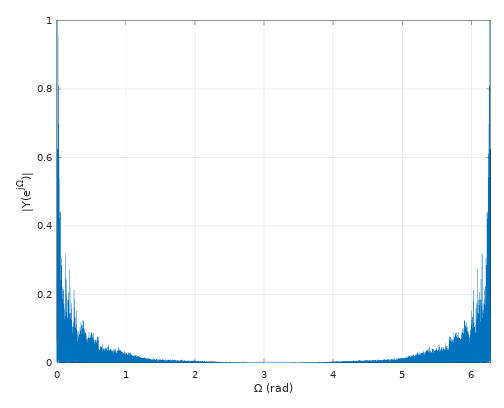
\includegraphics[width=0.3\textwidth]{images/spectre.png}
        \caption{Espectro de frequência $Y(j\Omega)$ em função de $\Omega$}
    \end{figure}

\item
    $y_{dec}(t)$ - sinal do arquivo 'queen\_I\_want\_it\_all.wav' amostrado em uma taxa Fs\_dec = Fs/6 = 7,35 kHz.

    Gráfico do espectro de frequência do sinal $y_{dec}(t)$:
    \begin{figure}[H]
    \centering
    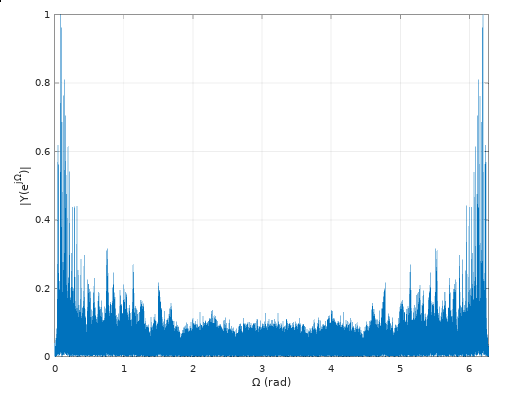
\includegraphics[width=0.3\textwidth]{images/spectre_dec.png}
        \caption{Espectro de frequência $Y_{dec}(j\Omega)$ em função de $\Omega$}
    \end{figure}
\break\vfill

\item
    Ouvi as musica

\item
    Gráficos das respostas em frequência $h(t)$:

    \begin{figure}[H]
    \centering
    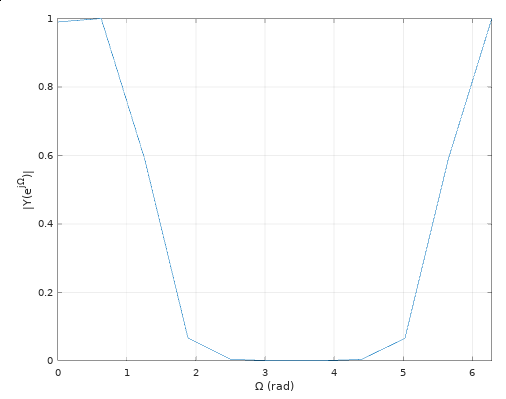
\includegraphics[width=0.4\textwidth]{images/h1.png}
        \caption{Filtro Kaiser $\omega_p = 0.45$ e $\omega_r = 2$}
    \end{figure}

    \begin{figure}[H]
    \centering
    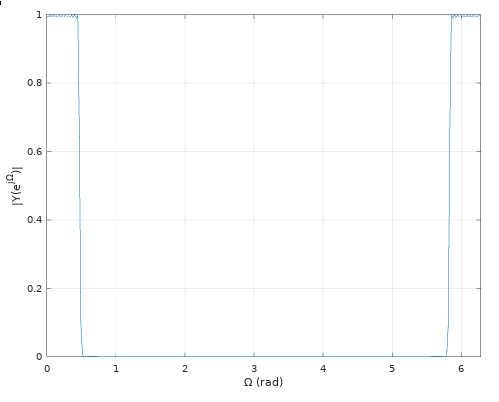
\includegraphics[width=0.4\textwidth]{images/h2.png}
        \caption{Filtro Kaiser $\omega_p = 0.45$ e $\omega_r = 0.5$}
    \end{figure}

    \begin{figure}[H]
    \centering
    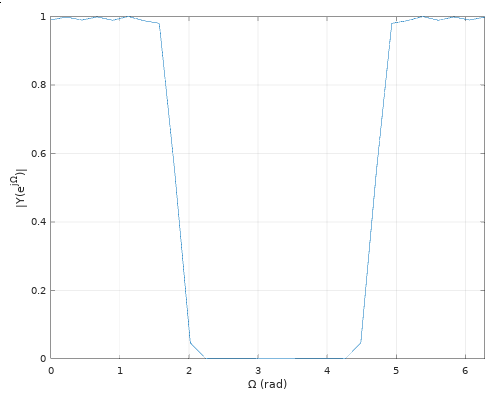
\includegraphics[width=0.4\textwidth]{images/h3.png}
        \caption{Filtro Kaiser $\omega_p = 1.5$ e $\omega_r = 2$}
    \end{figure}
\break\vfill

\item
    Gráfico da respostas em frequência de $h(t)*y(t)$:

    \begin{figure}[H]
    \centering
    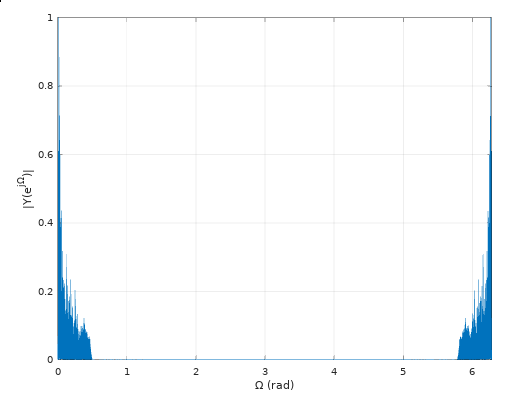
\includegraphics[width=0.5\textwidth]{images/conv_h.png}
        \caption{$y(t)$ aplicado o filtro Kaiser $\omega_p = 0.45$ e $\omega_r = 0.5$}
    \end{figure}

\item
    Gráfico da respostas em frequência de $h(t)*y(t)$ com M = 6:

    \begin{figure}[H]
    \centering
    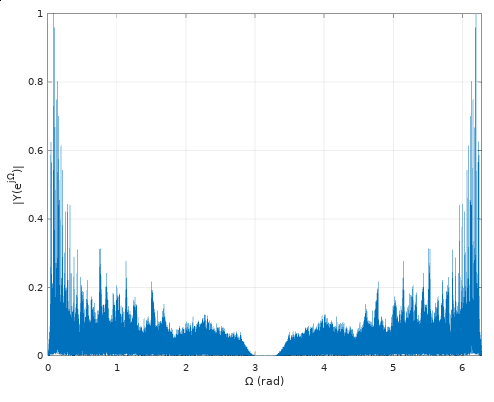
\includegraphics[width=0.5\textwidth]{images/resamp_after_filter.png}
        \caption{$y(t)$ amostrado com M=6 após ter sido aplicado o filtro Kaiser $\omega_p = 0.45$ e $\omega_r = 0.5$}
    \end{figure}

\end{enumerate}
\end{document}
